\documentclass{article}
\usepackage[utf8]{inputenc}
\usepackage{graphicx}
\graphicspath{ {./images/} }
\usepackage{amsmath}
\usepackage{hyperref}
%\usepackage[english]{babel}

\usepackage[left=2cm,right=1cm, top=2cm,bottom=2cm,bindingoffset=0cm]{geometry}

\renewcommand{\normalsize}{\fontsize{14}{18pt}\selectfont}

\title{Targeting the GPU with Kokkos}
\author{ Kamilla Faizullina}
\date{\empty}

\begin{document}


\maketitle
In this work, we implement a computation of the element matrices  with Kokkos and run the program on GPU and CPU to check the performance. Each element matrices is computed using its own Jacobian matrices (which are all the same, in our case). Therefore, we assume that each element computation is independent and we can use parallelism along axis linked to Number of elements. 

We use \href{https://www.nvidia.com/en-us/data-center/v100/}{NVDIA Tesla V100 Nvlink}. Memory bandwidth is  $900$ GB/s and the prformance is $7.8$  teraFLOPS for Double-Precision and $15.7$ teraFLOPS for Single-Precision.

 

\section{Implementation}
The matrices J (the inverse and transpose Jacobian ) and A (results) are stored as Kokkos::View type:

\begin{verbatim}
Kokkos::View<Number *[3][3], LayoutType, MemSpace> J("J", N);
Kokkos::View<Number *[4][4], LayoutType, MemSpace> A("A", N);
\end{verbatim}
Here $3$ dimensions in arrays: run-time, 2 compile-time.

We have $3\times3 + 4\times 4 = 25$ elements for two arrays for every computation. Therefore, I use the factor $25 N$ when calculate the performance.  

\section{ Performance for CPU and the GPU }
First, we run the program on GPU and CPU (for 4 and 16 processes) with default LayoutType. According to   \href{https://github-wiki-see.page/m/kokkos/kokkos/wiki/View}{documentation} , for execution space Cuda, the default layout is $LayoutLeft$. When the execution space is OpenMP, the layout is $LayoutRight$.

We measure the performance for both float and double types arrays.

Figure \ref{doubleorfloat} illustrates the obtained results. As we see, results from GPU are much better than from CPU on 16 processes. The computational performance for type $float$ are better than for $double$ in all cases. 

For large $N$, the obtained memory bandwidth on GPU with floats is approximately $650-750$ GB/s, which is close enough to the theoretical technical value $900$ GB/s (also, maybe calculation $25N$ does not take into account some other made actions). 


\begin{figure}[h]
	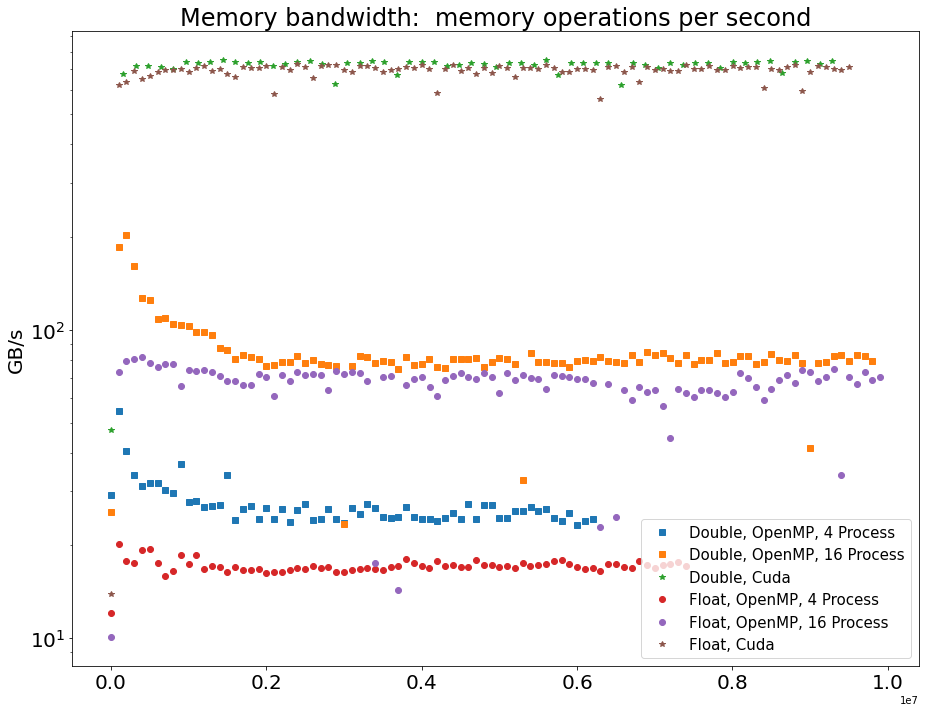
\includegraphics[scale=0.27]{memory.png} 
	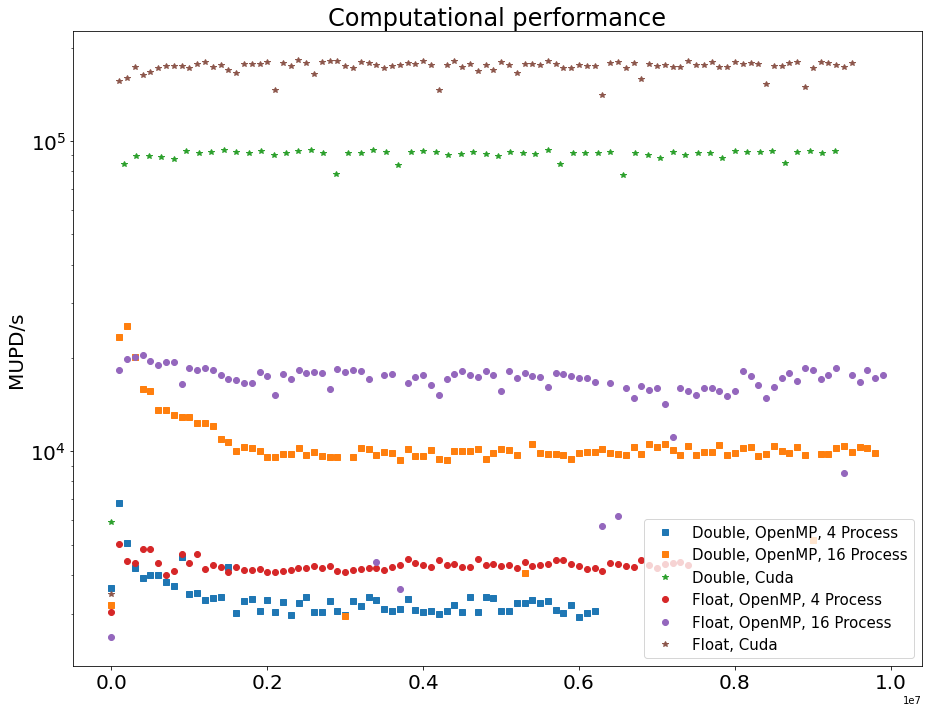
\includegraphics[scale=0.27]{comp.png}  
	\caption{ Measured performance for GPU and CPU (for 4 and 16 processes) using Kokkos with default layouts.  }
	\label{doubleorfloat}
\end{figure}

 \section{ LayoutRight vs LayoutLeft }
%\includegraphics[scale=0.6]{fow_prev_trim.png}
 \begin{figure}[h]
 	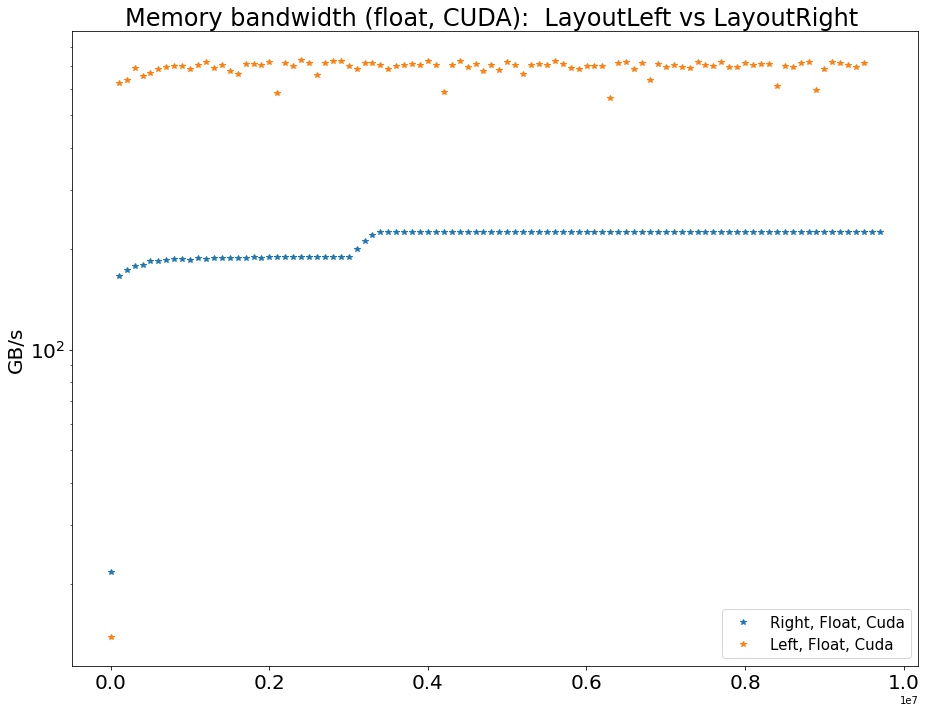
\includegraphics[scale=0.27]{memory_lr_cuda.png} 
 	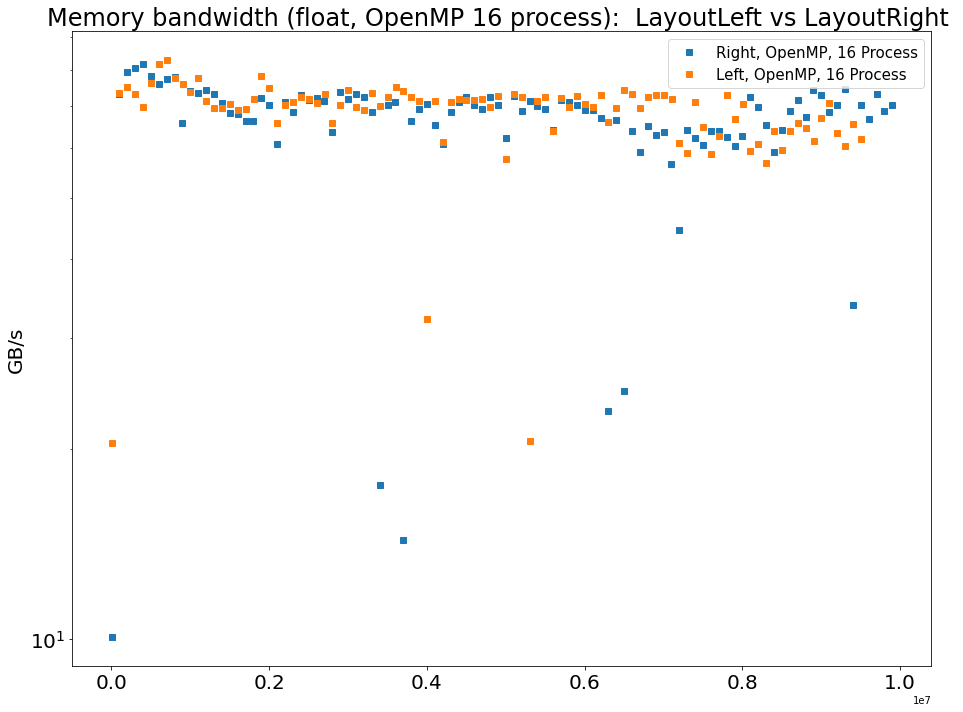
\includegraphics[scale=0.27]{memory_lr_openmp_16.png}  
 	\caption{ Measured performance for GPU and CPU (for 16 processes) using Kokkos with LayoutLeft and LayoutRight.  }
 	\label{leftorright}
 \end{figure}
Kokkos allows to choose manually the Layout in Arrays. LayoutLeft is  column-major layout and LayoutRight is row-ordered. 
Figure \ref{leftorright} shows how choice of Layout affect the performance. As we can see, for GPU the leftlayout choice is better. Therefore, it is not surprising that for simple parallels the LayoutLeft is defoult choice on Cuda. For runs with OpenMP, the difference is not significant. However, it was expected that the LayoutRight would outperform. 
%\begin{thebibliography}{9}

 \section{Timing}
 \begin{figure}[h]
 	\centering
	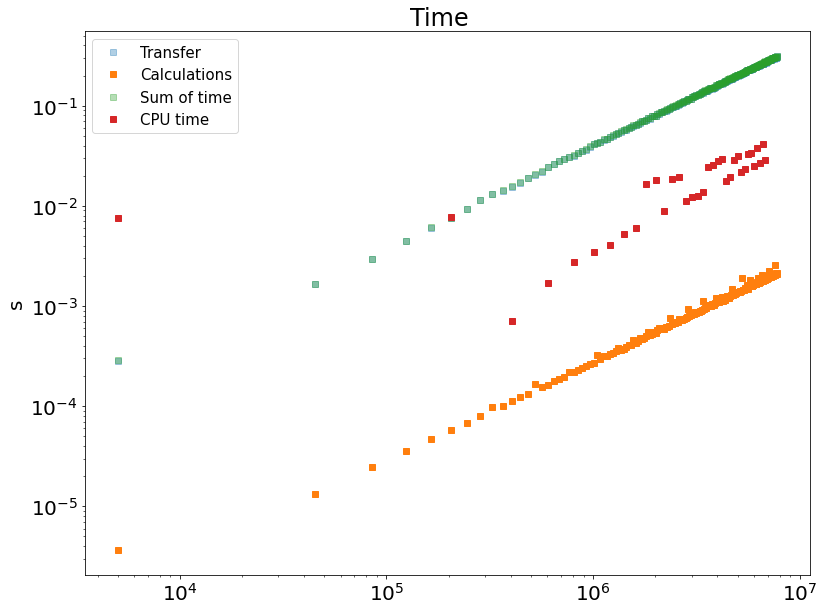
\includegraphics[scale=0.37]{time.png}  
	\caption{ Measured time for transfer and calculations.  }
	\label{time}
\end{figure}
%\end{thebibliography}
Figure \ref{time} shows how much time transferring data between host and device costs for GPU. The total time is mostly time for copy. The difference approximately 100 times. In general, running CPU was less time-consuming because there is no data transfer. 

I suppose that for one-time operations we should use CPU to save time on transferring. For iterative actions, we should use GPU (however, it depends on the number of iterations). if iterations less than 100 I am not sure that we would enough. 

\end{document}
